\documentclass[a4paper, 11pt]{article} % Font size (can be 10pt, 11pt or 12pt) and paper size (remove a4paper for US letter paper)

\usepackage[protrusion=true,expansion=true]{microtype} % Better typography
\usepackage{graphicx} % Required for including pictures
\usepackage{wrapfig} % Allows in-line images
\usepackage{enumitem} %%Enables control over enumerate and itemize environments
\usepackage{setspace}
\usepackage{amssymb, amsmath, mathrsfs,mathabx} %%Math packages
\usepackage{stmaryrd}
\usepackage{mathtools}
\usepackage{multicol} 
\usepackage{mathpazo} % Use the Palatino font
\usepackage[T1]{fontenc} % Required for accented characters
\usepackage{array}
\usepackage{bibentry}
\usepackage{prooftrees} 
\usepackage[round]{natbib} %%Or change 'round' to 'square' for square backers
\setcitestyle{aysep=}
% \usepackage{fitchproof} 

% \linespread{1.05} % Change line spacing here, Palatino benefits from a slight increase by default

\newcommand{\tuple}[1]{\langle#1\rangle} %%Angle brackets
\newcommand{\set}[1]{\lbrace#1\rbrace} %%Set brackets
\newcommand{\abs}[1]{|#1|} %%Set brackets
\newcommand{\interpret}[1]{\llbracket#1\rrbracket} %%Double brackets
\newcommand{\N}{\mathbb{N}}
\newcommand{\D}{\mathbb{D}}
\newcommand{\Z}{\mathbb{Z}}
\renewcommand{\Pr}{\mathbb{P}}
\newcommand{\Q}{\mathbb{Q}}
\newcommand{\R}{\mathbb{R}}
\newcommand{\B}{\mathfrak{B}}

\makeatletter
\renewcommand\@biblabel[1]{\textbf{#1.}} % Change the square brackets for each bibliography item from '[1]' to '1.'
\renewcommand{\@listI}{\itemsep=0pt} % Reduce the space between items in the itemize and enumerate environments and the bibliography

\renewcommand{\maketitle}{ % Customize the title - do not edit title and author name here, see the TITLE block below
\begin{flushright} % Right align
{\LARGE\@title} % Increase the font size of the title

\vspace{10pt} % Some vertical space between the title and author name

{\@author} % Author name
\\\@date % Date

\vspace{-30pt} % Some vertical space between the author block and abstract
\end{flushright}
}

%----------------------------------------------------------------------------------------
%	TITLE
%----------------------------------------------------------------------------------------

\title{\textbf{Omega Sequences}} % Subtitle

\author{\textsc{Paradox and Infinity}\\ \em Benjamin Brast-McKie} % Institution

\date{\today} % Date

%----------------------------------------------------------------------------------------

\begin{document}

\maketitle % Print the title section

\thispagestyle{empty}

%----------------------------------------------------------------------------------------

\section*{Ordinals into Obscurity?}

\begin{itemize}
  \item[\it Definition:] Let $\B_\alpha = 
    \begin{cases}
      \N                                            & \text{if } \alpha = 0\\
      \wp(\B_\beta)                                 & \text{if } \alpha = \beta'\\
      \bigcup \set{ \B_\gamma : \gamma <_o \alpha } & \text{otherwise.} 
    \end{cases}$
  \item[\it Obscurity:] But all of this is only studied within set theory.
    \item Neither standard mathematics nor the sciences need ordinals beyond $\omega$ nor cardinalities beyond the continuum. 
    \item But there are puzzles that arise even for $\omega$ sequences. 
    \item Simplest case of the infinite worth exploring.
  \item[\it Motivations:] Why care about all of this?
    \item Because we can.
    \item Because it's awesome (in the religious sense).
    \item We are probing the limits of what is thinkable, not useful.
\end{itemize}



\section*{Zeno's Analysis}

\begin{itemize}
  \item[\it Dichotomy Paradox:] ``That which is in locomotion must arrive at the half-way stage before it arrives at the goal.'' -- Aristotle, Physics VI:9, 239b10
  \item[\it Infinite Task:] Doing infinitely many tasks, each taking a non-zero amount of time.
    \item Some infinite tasks are cannot be performed in a finite amount of time.
  \item[\bf Question:] What about infinite tasks with strictly decreasing times for each task?
    \item The harmonic series is a counterexample: $\sum_{n=1}^\infty \frac{1}{n}$ diverges.
    \item $H = 1 + \frac{1}{2} + \frac{1}{3} + \frac{1}{4} + \frac{1}{5} + \frac{1}{6} + \ldots \geq 1 + \frac{1}{2} + \frac{1}{4} + \frac{1}{4} + \frac{1}{6} + \frac{1}{6} + \ldots = \frac{1}{2} + H$.
  \item[\it Super Task:] An infinite task that is performed in finite time. 
    \item Example: walking across the room since $\sum_{n=1}^\infty \frac{1}{2^n}$ converges to 1.
    \item $f(1)=\frac{1}{2}$, $f(2)=\frac{3}{4}$, $f(3)=\frac{7}{8}$, $f(4)=\frac{15}{16}$, \ldots, so $f(n)=1-\frac{1}{2^n}$.
    \item \mbox{For any $\epsilon > 0$, there is some $n \in \N$ where $\abs{1-f(m)} < \epsilon$ for any $m > n$.}
  \item[\it Paradox:] So there are super tasks, though this would have surprised Zeno.
    \item It took the development of analysis in 17th century to solve.
    \item Analysis was not put on solid foundations until the 19th century by Bolzano, Cauchy, and Weierstrass.
    \item Poster child of illuminating paradoxes, but not all are like this.
\end{itemize}




\section*{Thomson's Lamp}

\begin{itemize}
  \item[\it Descriptions:] 60s (off); 30s (on); 15s (off); \ldots
    \item Compare $f(n)=\texttt{sin}(\frac{\pi}{1-x})$ to $g(n)=\texttt{sin}(\frac{\pi}{1-x})(1-x)$.
      \begin{multicols}{2}
        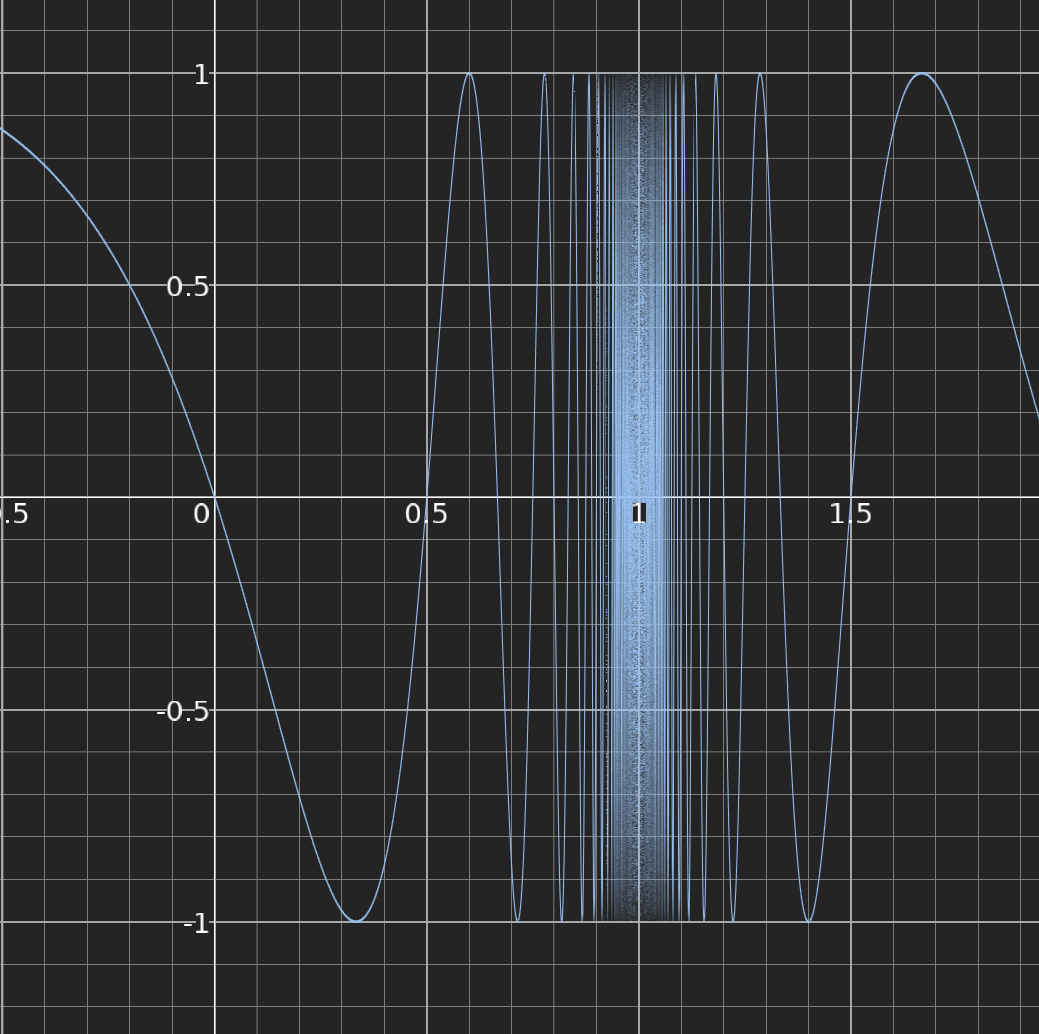
\includegraphics[scale=.16]{Lamp}
        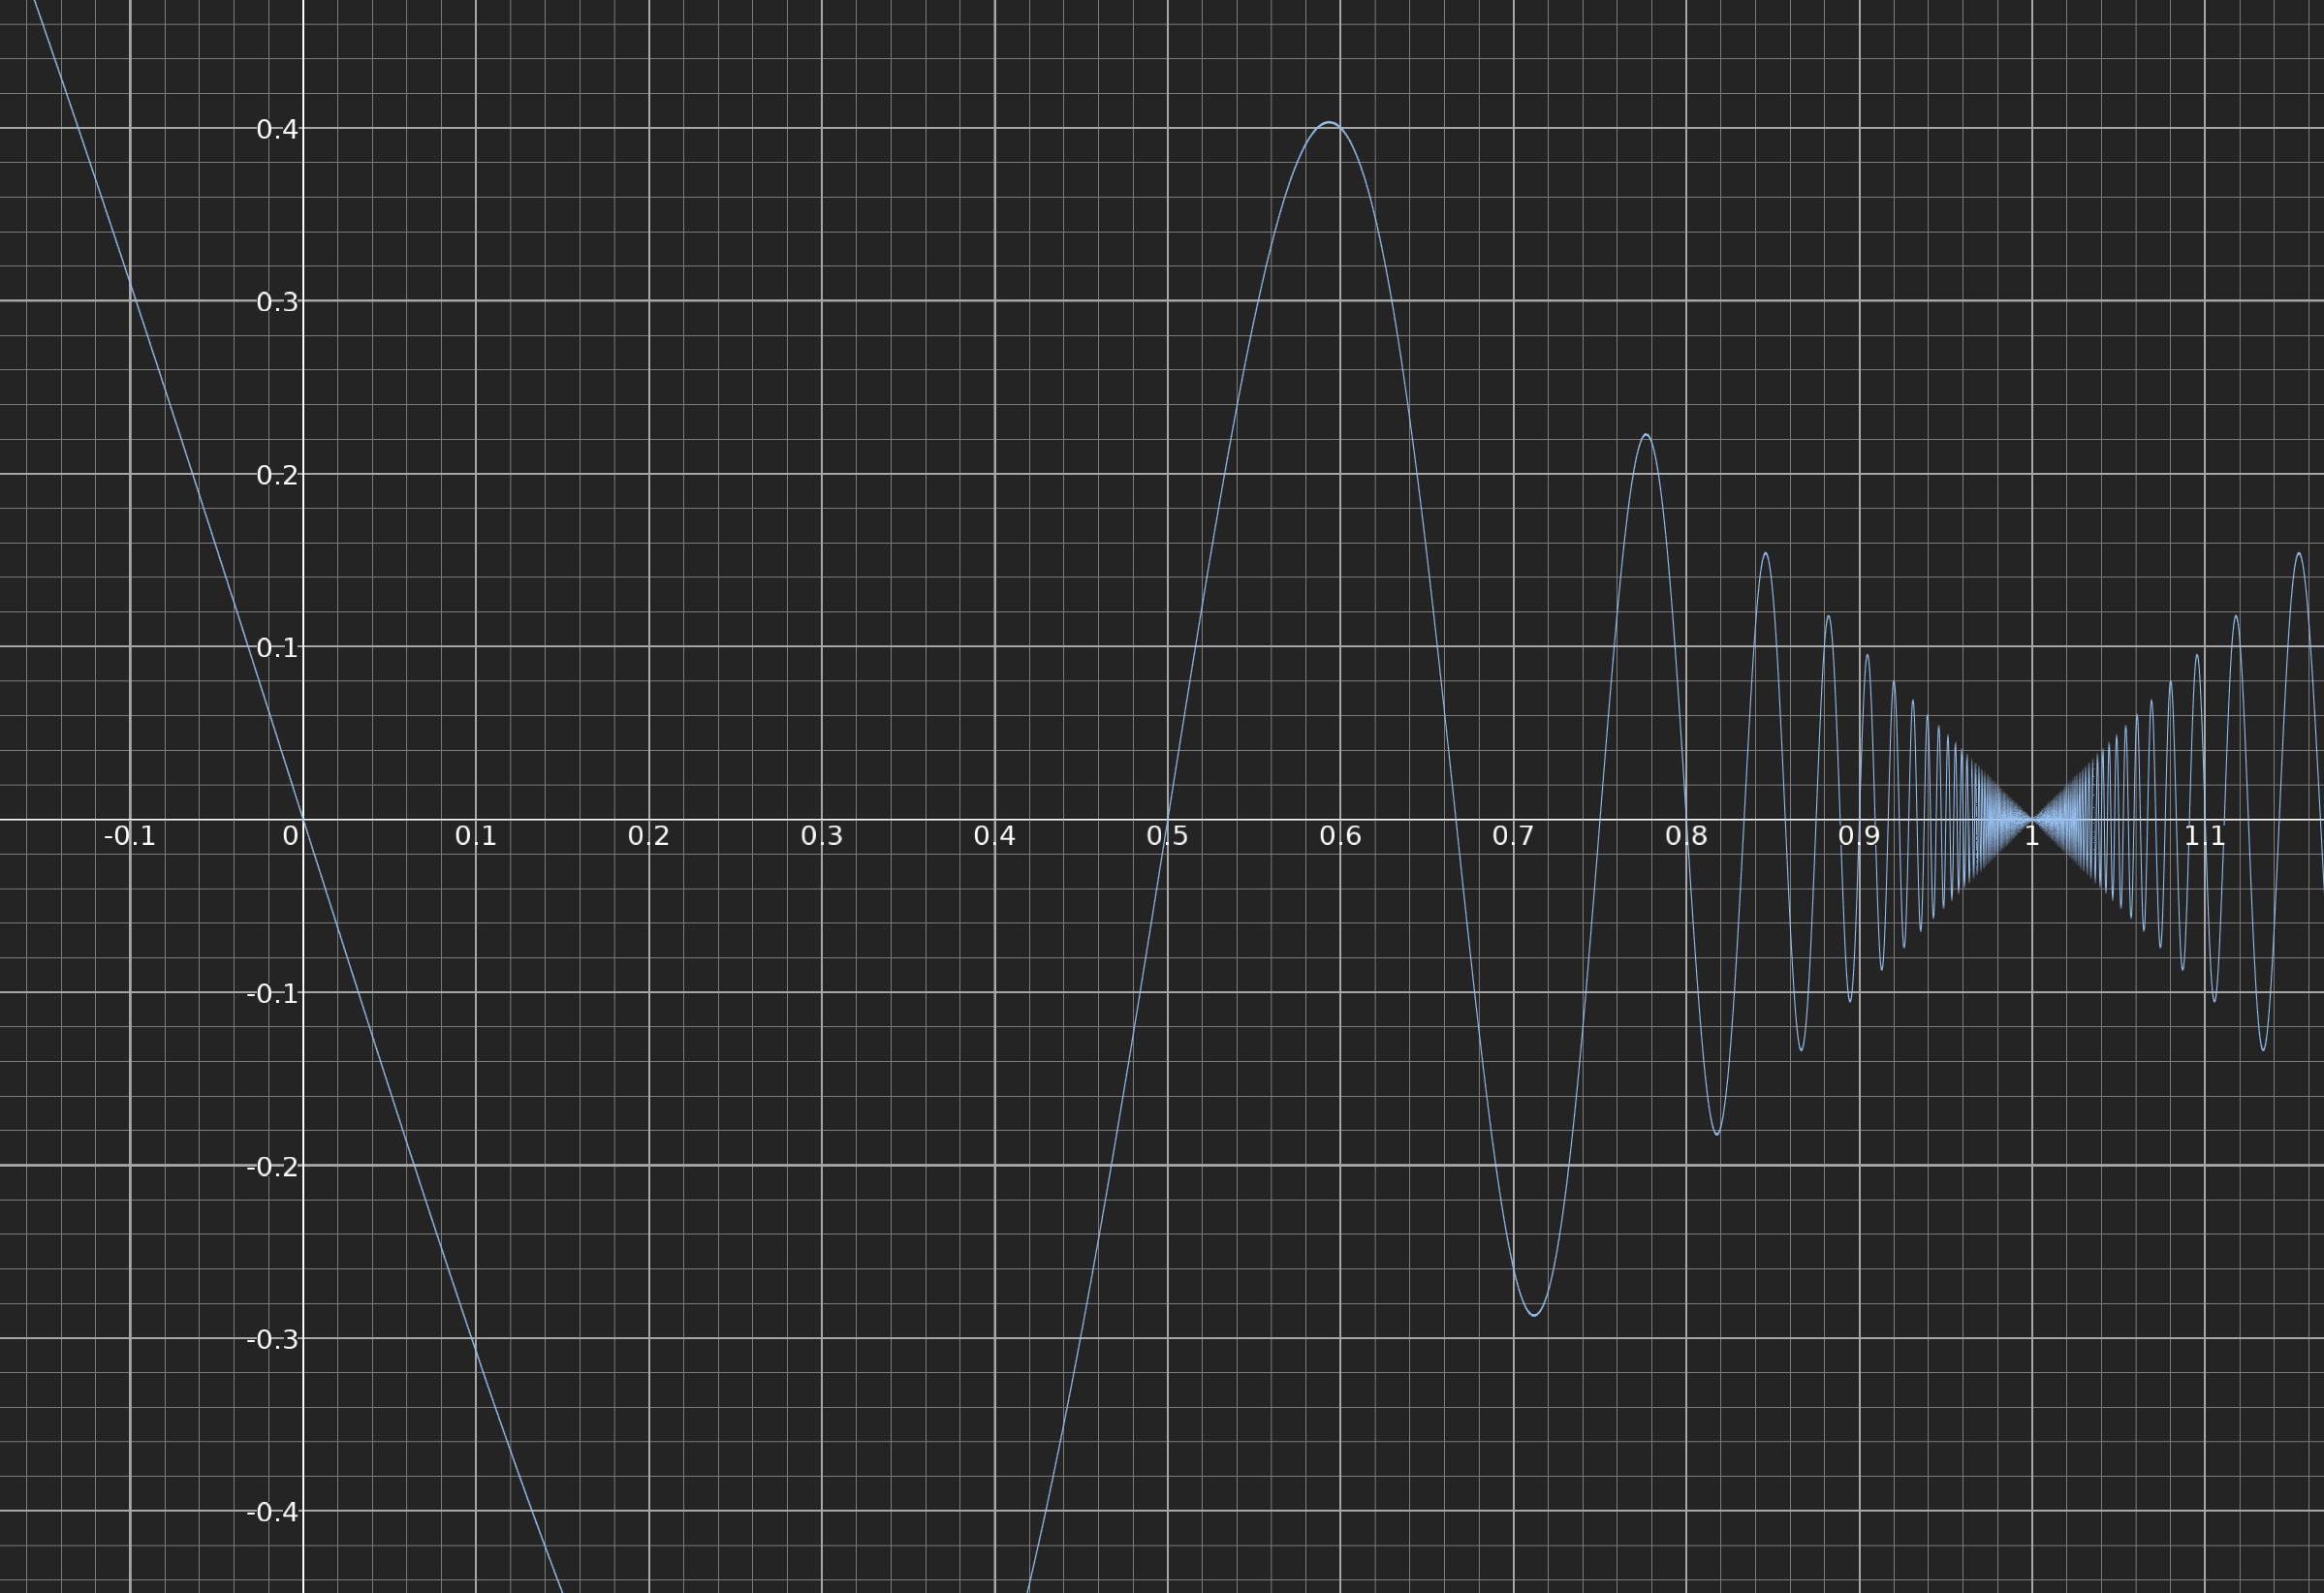
\includegraphics[scale=.1]{LampDec}
      \end{multicols}
    \item No continuous function satisfying the description is defined at $n=1$.
    \item Subsequences of a convergent sequence converge to the same limit as the original, so neither the above nor $1, -1, 1, -1, \ldots$ converge.
\end{itemize}





\section*{Demon's Game}

\begin{itemize}
  \item[\it Setup:] ``As long as only finitely many of you say \textit{aye}, each of you will receive as many gold coins as there are people who said \textit{aye}.'' 
    \item Assumes everyone is ``optimally rational'' and cannot collaborate.
    \item Is maximizing really ``optimally rational'' in this scenario?
  \item[\it Individual Version:] ``If you answer \textit{aye} at most finitely many times, you will receive as many gold coins as the \textit{aye}-answers that you give.''
    \item Assumes no diachronic collaboration between time-slices. 
    \item It is wrong to assume that the will is unable to persist across times.
  \item[\it Video Rental:] \$5 to rent, \$2 late fee, but it is always worth it to Daniel to pay the fee.
    \item This is not a paradox, just a problem that Daniel has.
    \item Also a problem for a theory of rationality that takes Daniel to be ideally rational given his preferences at each time.
  \item[\it Buridan's Ass:] Compare infinite ever larger bales of hay to the duplicate bale case.
    \item The ass does not starve, but not because of its sins against rationality.
    \item We can choose between duplicates/an arbitrary cut-off point.
\end{itemize}


\end{document}


